%!TEX root = thesis_main.tex

\chapter{Testing and Analysis of single-stage Cycloid}\label{ch:single}
%Give and Overview of Chapter 3

There is a gap in the literature for the in-use efficiency and lifetime characteristics of cycloidal reducers of the compact design that was presented in Chapter \ref{ch:design_1s}. Previously, the longest set of test data for a compact cycloid was 80 minutes. This work aims to develop an understanding of the in-use characteristics of the single-stage compact design cycloid reducer in both efficiency and the initial analysis of lifetime for a cycloid of this type. Therefore, the single-stage design previously discussed was run through a long duration life-cycle with efficiency testing performed periodically to understand these pertinent characteristics. The actuator was run for over 300 hours with 130k output revolutions. The peak efficiency achieved through this time was 81\% which shows this actuator is competitive in efficiency with a harmonic drive. In addition, no appreciable degradation of performance was seen from break in until testing completion, showing the actuator's lifetime easily exceeds the current testing time.  

This work has been submitted to the International Conference on Robotics and Automation, ICRA with the title ``Cycloidal Geartrain In-Use Efficiency Study.'' Portions of this section are taken directly from this publication. This chapter will first cover the experimental test setup in Section \ref{ch:single:test_setup}. The results of this testing are presented in Section \ref{ch:single:eff_results}. An analysis of the wear of the components is presented in Section \ref{ch:single:wear_analysis}. Finally, a discussion of these results is given in Section \ref{ch:single:discussion}.

\section{Test Setup} \label{ch:single:test_setup}
%Give the test setup for the single-stage, basically pull the info from the paper 

The intent of testing the cycloidal drive is to experimentally determine and compare the in-use efficiency results to the published performance data for a comparable harmonic drive.
To accomplish this, the actuator was mounted to a Futek TF600 5000inlb load cell to measure output torque of the actuator.
The load cell signal was collected through a analog to digital converter and converted to standard units on the motor driver.
A verification of torque readings was completed using a calibrated torque wrench to ensure accuracy of the conversion.
Load was regulated by a Magtrol HB-1750 hysteresis brake.
A 36:1 speed increase was added via three chain stages between the output of the actuator and the hysteresis brake to achieve the desired applied loads.
The hysteresis brake was powered using a separate 24V Lambda-TDK power supply that was controlled through a RS-485 communication link to the test computer.
NASA's 'turbodriver' motor driver was used for commanding motor currents.
The motor driver was powered by a TDK-Lambda 12V supply for logic power and a TDK-Lambda 150V and 5A supply for high voltage power.
A hysteresis current controller was used on the motor drive to accurately provide torque producing current to the motor.
The motor driver monitored the actuator power by measuring torque from the load cell and speed with an incremental encoder located at the actuator motor shaft.
The test computer monitored the high voltage supply and recorded voltage and current to determine input power to the system and received data from the motor driver to calculate output power.
The test setup is shown in Fig \ref{fig:test_setup}.

\begin{figure}[t]
   \centering
   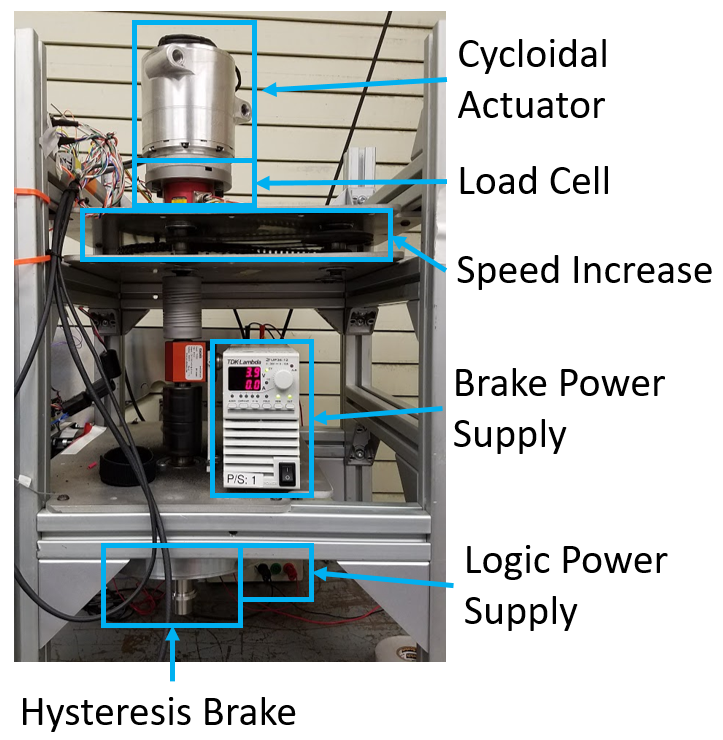
\includegraphics[width=0.75\linewidth]{fig/test_stand}
   \caption{Experimental Test Setup.
   The cycloid actuator is mounted to structure via the load cell.
   There is a speed increase so the brake can generate enough torque on the system.
   Not pictured is the controlling computer, motor driver, and high voltage supply.}
   \label{fig:test_setup}
\end{figure}

Due to the tightly integrated actuator design, the motor and cycloid cannot be separated to purely isolate the losses in the cycloid.
The efficiency map of the motor over its torque and speed range was provided by Parker Motors.
For calculation purposes, this table is used as a lookup table for efficiency of the motor given the current motor velocity and rms input current.
While this does generate a level of uncertainty in the data, these motors are mass manufactured and defects are assumed to be small.
The error in the motor efficiency map is assumed to be small and would not influence the perceived trends and results.
Power losses in the motor driver were also taken into consideration by calculating power losses in the IGBT that drives the motor.
Instantaneous current draw and a switching frequency of 12 kHz were used for the calculation, neglecting small leakage losses \cite{ref:IGBTPower}.

\begin{figure}[t]
   \centering
   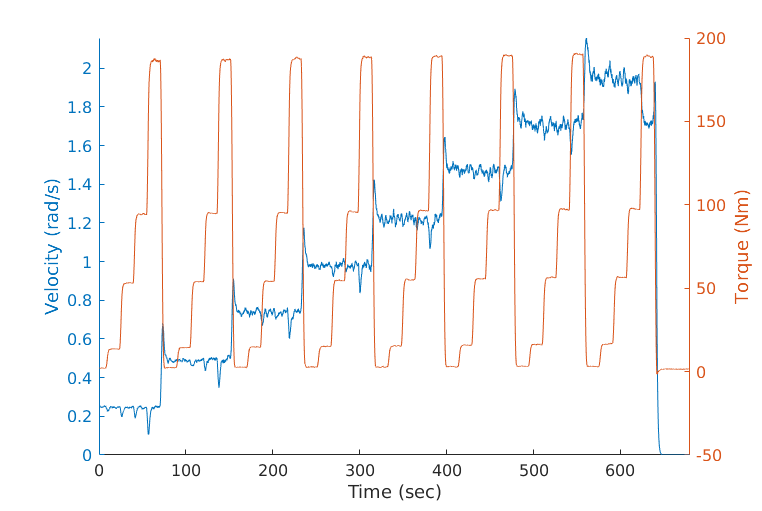
\includegraphics[width=\linewidth]{fig/eff_test_profile_v4}
   \caption{Testing profile for efficiency.
   At each speed step, torque is ramped up through five different levels, then the speed is increased.
   At the last step, the maximum of the supply was reached so motor velocity dropped.}
   \label{fig:eff_profile}
\end{figure}

The system was tested in two separate ways, an efficiency cycle and a long term drive cycle.
The efficiency cycle was run multiple times throughout the lifetime testing, first after the actuator achieved steady state efficiency, and again after each 100 hours of testing.
For the efficiency cycle, the actuator is subjected to eight velocity steps increasing 0.25 rad/s each time.
In each velocity step, the torque is ramped up and maintained for 15 seconds at values of 1Nm, 15Nm, 52Nm, 94Nm, and 189Nm.
This testing profile can be seen in Fig \ref{fig:eff_profile}.
The long term drive cycle was run continuously each day for 6 to 12 hours with the duty cycles shown in Table \ref{table:long_run}.
The total runtime of the system, not including the initial checkout and verification of the actuator, has been 303 hours.

\begin{table}[t]
  \vskip0.2cm
  \caption{Long Run Drive Cycle}
  \label{table:long_run}
  \begin{center}
    \vskip-0.2cm
    \begin{tabular}{|c||c||c|}
    \hline
    Time (s) & Velocity (rad/s) & Torque (Nm)\\
    \hline
    150 & 1.0 & 0.0\\
    \hline
    150 & -1.0 & 0.0\\
    \hline
    60 & 0.5 & 26.0\\
    \hline
    60 & -0.5 & 26.0\\
    \hline
    150 & 1.5 & 10.0\\
    \hline
    150 & -1.5 & 10.0\\
    \hline
    30 & 1.0 & 50.0\\
    \hline
    30 & -1.0 & 50.0\\
    \hline
    300 & 0.5 & 18.0\\
    \hline
    300 & -0.5 & 18.0\\
    \hline
    \end{tabular}
  \end{center}
\end{table}

It should be noted that the actuator was used briefly in the robot validation after initial development and construction of the prototype wheel module.
The total time of use was approximately three hours.
Afterwards, it was removed from the wheel module and subjected to the characterization that is discussed in this work.
The motor has a continuous current rating of 4.3 A\textsubscript{rms} and a peak rating of 15A\textsubscript{rms}.
The actuator was designed to be liquid cooled to allow operations above the continuous values, but this could not be achieved during testing.
For long duration testing, the torque values were decreased to avoid thermal issues.
The motor was tested to approximately 6A\textsubscript{rms} during efficiency testing due to the limit of the power supply.
Also, the motor driver's rated limits are 150V, therefore the actuator's maximum rated speeds could not be tested.
The nominal cycle of the actuator as seen in Table \ref{table:duty_cycle} is still achievable and has been tested.



\section{Results} \label{ch:single:eff_results}
%Discuss the results that we achieved 
% - burn in time 
% - efficiency over the current run time 
% - specific efficiency runs
% - compare to the "expected" efficiency from the rolling anlaysis 

Duty cycle testing was performed first on the actuator.
These tests were done at lower torques to prevent the motor from overheating to allow extended duration testing.
The total test time prior to these duty cycle tests was approximately 5.2 hours to bring up and check out the actuator testbed system.
Once this checkout was complete, the 300 hours of duty cycle testing were conducted over the course of 39 days with the drive cycle presented in Table \ref{table:long_run}.
Three of the torque/speed combinations in forward and reverse are plotted on Fig \ref{fig:long_run} to show the general characteristic trends seen in actuator performance.

\begin{figure}[!b]
   \centering
   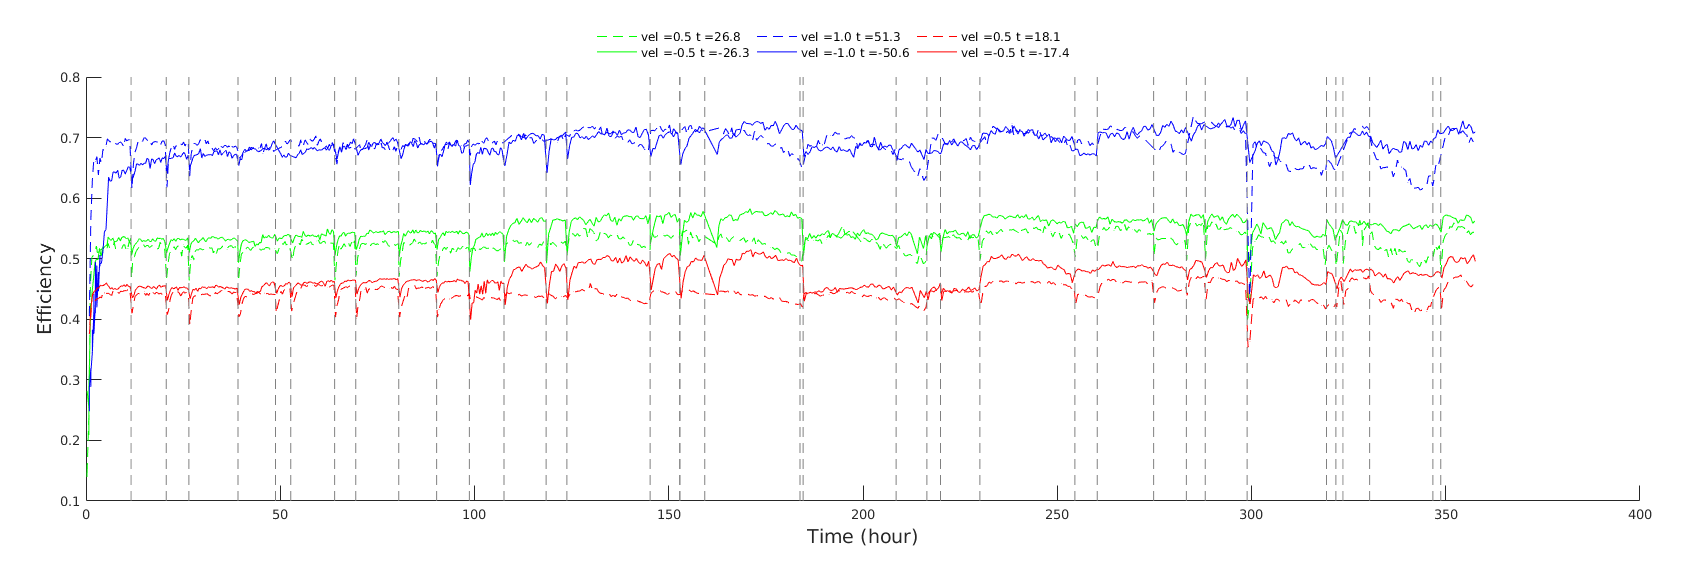
\includegraphics[width=\linewidth]{fig/total_runtime}
   \caption{Efficiency over time for three different speed/torque profiles during the drive cycle.
   The forward motion can be seen with the dotted line, reverse with the solid line.
   Testing transitions from day to day are denoted with vertical dotted lines.
   At the onset of testing, visible efficiency gains are made.
   As each day begins, there is a clear warm-up period before steady state.
   }
   \label{fig:long_run}
\end{figure}
\todo[inline]{fix the legend to be a real size}

After the break in period and steady state performance was achieved, a profile of speeds and torques (see Fig \ref{fig:eff_profile}) were run on the actuator to show the relationship between speed, torque, and efficiency.
This profile was run three times and the results at each torque and speed combination were averaged. The first efficiency cycle was run as seen in Fig \ref{fig:eff_results}. Efficiency cycles were run after each subsequent 100 hours of testing to understand performance over time. The final efficiency test is shown in Fig \ref{fig:eff_results_final}.

\begin{figure}[h]
   \centering
   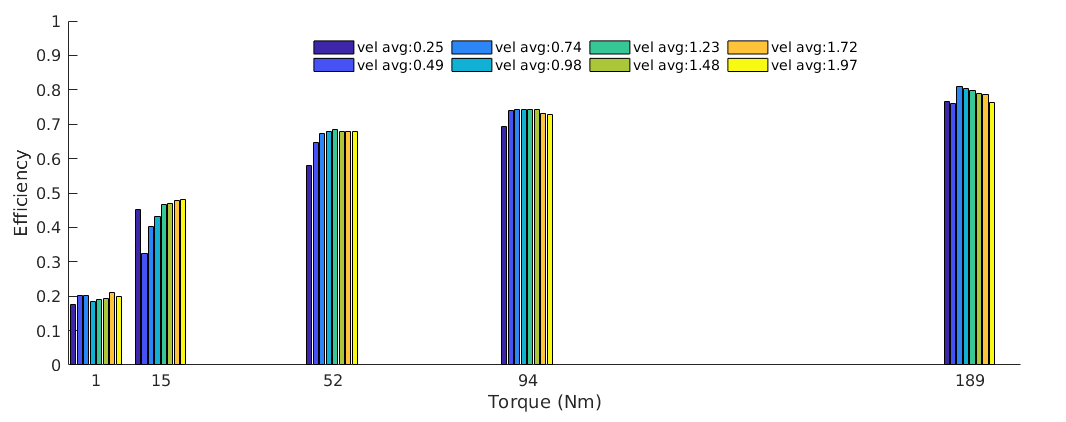
\includegraphics[width=0.8\linewidth]{fig/eff_test_bar_plot_v3}
   \caption{Efficiency of the single-stage cycloid after 100 hours of testing. Grouping of average efficiencies at each torque step.
   Efficiency depends heavily on torque, and slightly on speed.}
   \label{fig:eff_results}
\end{figure}

\begin{figure}[h]
   \centering
   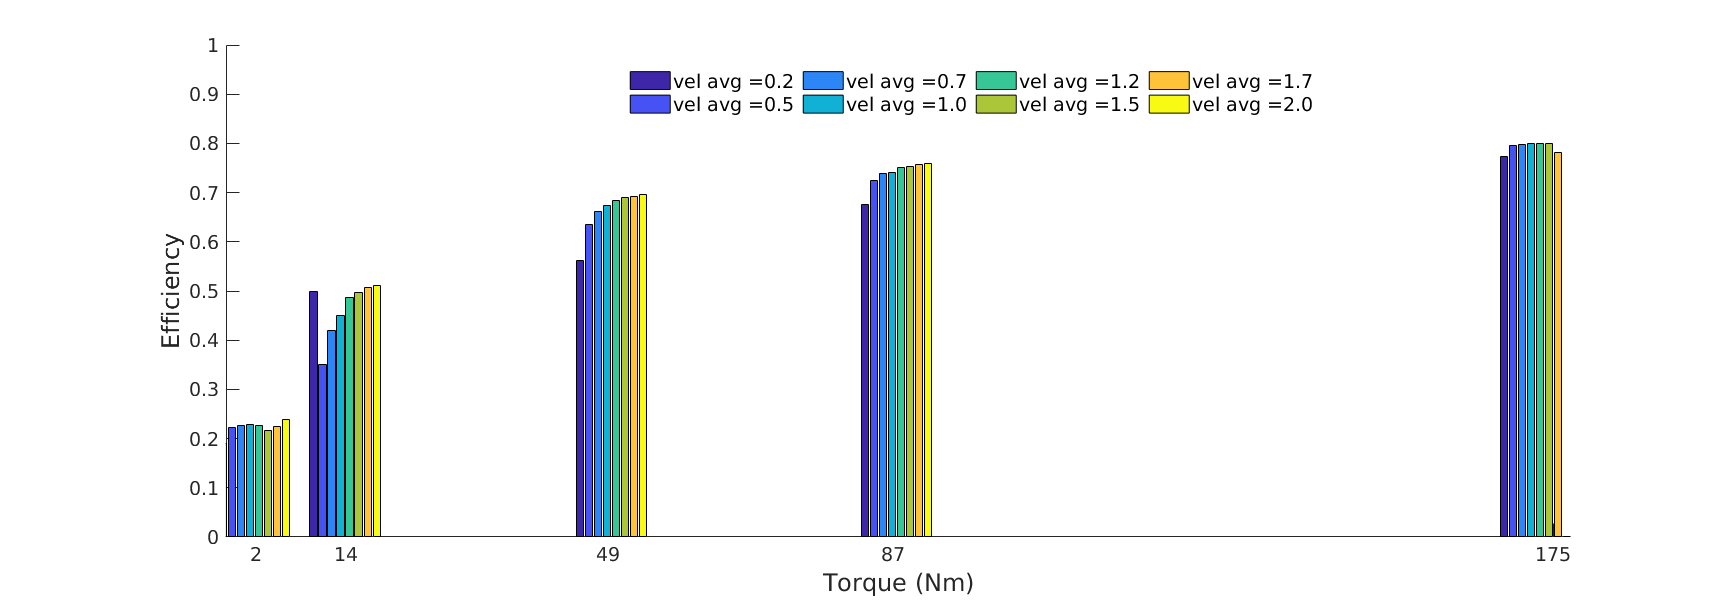
\includegraphics[width=0.8\linewidth]{fig/eff_final}
   \caption{Efficiency of single-stage cycloid after 300 hours of testing. No appreciable loss of efficiency after 129k revolutions. TODO - make the legend look the same as the one above }
   \label{fig:eff_results_final}
\end{figure}
\todo[inline]{make the legend size reasonable and the same}

\section{Wear Analysis} \label{ch:single:wear_analysis}
% Look at the pictures that we took to say "check it out, this thing can probably go for a lot longer based on how well it's done so far."
% The only real thing to look at is those plastic pieces and talk about uneven wearing on the output pins. 

After completion of the 300 hours, and 129k cycles of testing, the actuator was disassembled to qualitatively analyze the wear patterns on the cycloid. This analysis gives an interesting look as to the wear and potential lifetime of the system. 

The first note is that the grease used, Red 'N Tacky from Lucas Oil, had turned a much darker color, nearly black. The system with the output pins and plate removed can be seen in Fig \ref{fig:single_full}. After removing the individual pieces and cleaning, the wear patterns in the system become clear. The cycloid plate, Fig \ref{fig:cycloid_plate}, shows smoothing of the peaks of the lobes on the plate, where they interact with the housing pins, but shows no wear deeper in the pockets. This indicates that the machining tolerances were such that these never interacted with the pins. The wear along the faces of each lobe were consistent around the profile, suggesting each lobe carried load at some point in each cycle. Additionally, the internal holes for the output pins shows relatively even wear. These results are typical for each of the three cycloid plates. 

\begin{figure}[t]
   \centering
   \includegraphics[width=0.4\linewidth]{fig/single_full}
   \caption{The single-stage cycloid with the output plate removed. The initially red grease has been turned nearly black through operation, likely due to metal deposits from the wearing in of the system.}
   \label{fig:single_full}
\end{figure}

\begin{figure}[!b]
   \centering
   \includegraphics[width=0.8\linewidth]{fig/cycloid_plate}
   \caption{The profile of one of the cycloid plates from the single-stage actuator. Each lobe shows smoothing along convex portion of the lobe and no wear along the concave portion. The wear is also uniform around the profile, showing relatively even load distribution around the profile during operation.}
   \label{fig:cycloid_plate}
\end{figure}


Three of the housing pins can be seen as an example in Fig \ref{fig:single_housing_pins}. The wear on these pins is uniform all the way around the pin. This shows that the pin was in fact rotating in the housing during operation, as determined by the sliding analysis in Section \ref{ch:design:pin_roll_1s:sliding_equations}. These three pins are also indicative of the other 57 pins, as each had relatively uniform wear around the profile. This, coupled with the cycloid plate, suggests that during the bulk of operation, the load was shared amongst all of the lobes and pins, rather than a small set of them. This potentially could have happened during the break in period of the system as well. 

\begin{figure}[t]
   \centering
   \includegraphics[width=0.3\linewidth]{fig/housing_pins}
   \caption{The pins that rest in the housing for the single-stage cycloid. The pins showed uniform wear around their diameter and across the pins, suggesting that the load was shared relatively equally around the diameter of the actuator.}
   \label{fig:single_housing_pins}
\end{figure}


The output pins can be seen in Fig \ref{fig:single_output_pins}. The output pins were fixed in the output plate and could not roll, which is evident in their wear pattern. One side of the pin has wear, while the other still has the original black oxide coating. This result makes sense since the pin is only in contact with the cycloid plate through half of the revolution. One interesting result from this though is that some pins show much more wear than others, indicating that fewer output pins were carrying load than the maximum possible, potentially resulting in more losses. A more optimal design of this system would allow these pins to roll in their housing to wear more evenly and in a potentially lower friction interaction. 

\begin{figure}[!b]
   \centering
   \includegraphics[width=0.7\linewidth]{fig/output_pins}
   \caption{The single-stage cycloid output pins. The pins did not rotate in their housing, so the wear is uneven around the diameter of the pin. The pins also show uneven wear from pin to pin, suggesting load was not carried equally among the pins during operation.}
   \label{fig:single_output_pins}
\end{figure}

\section{Discussion} \label{ch:single:discussion}
% Summary
% single-stage reductions built in this style can result in highly competitive efficiency ratios and 2x specific torque. You still have to deal with torque ripple and a little bit of backlash (unmeasured), but if you can handle those, drop these bad boys in. 

The efficiency of the system is dependent on the torque through the gearbox as shown in Fig \ref{fig:eff_results_final}.
This contradicts previous studies that suggested that cycloidal drives have a constant efficiency across the torque range.
There is also a much less pronounced relationship between the velocity and the cycloid efficiency that can be noted in the torque bands.
This result suggests that the cycloid efficiency behaves more like a planetary or harmonic drive gearbox in its efficiency profile.
A comparison of cycloid, harmonic, and planetary efficiency profiles can be seen in Fig \ref{fig:eff_comp}.
The figure shows the efficiency for a harmonic drive CSF-45-50-2UH-LW \cite{ref:harmonic_sheet} which has a comparable ratio and torque capability to the tested cycloid and weighs 5.1kg, and a representative planetary efficiency curve from the engineers at Maxon Motor.
If backlash is acceptable in a system, a cycloidal drive can provide similar or better efficiency profiles to a harmonic drive while providing a potential 2x increase in specific torque (Nm/kg).

\begin{figure}[h]
   \centering
   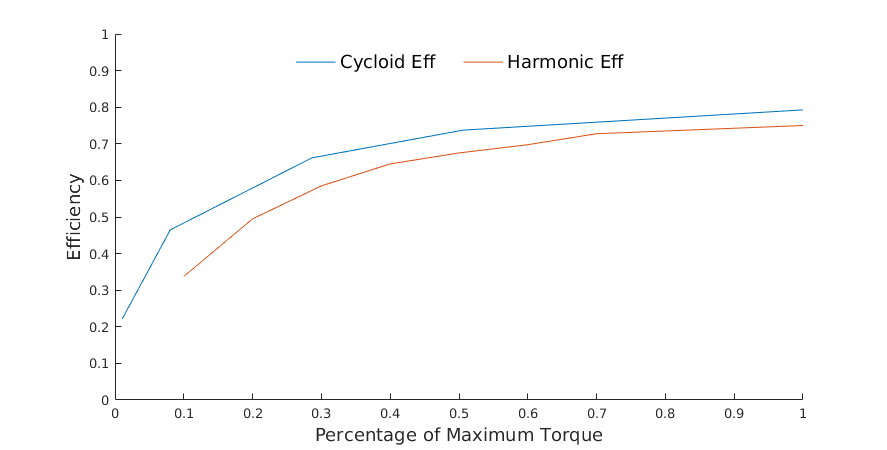
\includegraphics[width=0.7\linewidth]{fig/eff_comp_v3}
   \caption{Comparison of efficiency over maximum torque rating of the tested cycloid, a comparable harmonic drive, and a theoretical planetary gearset.
   The cycloid exhibits the same efficiency increase over torque range and has a comparable and slightly higher efficiency than the harmonic.}
   \label{fig:eff_comp}
\end{figure}

\begin{figure}[h]
   \centering
   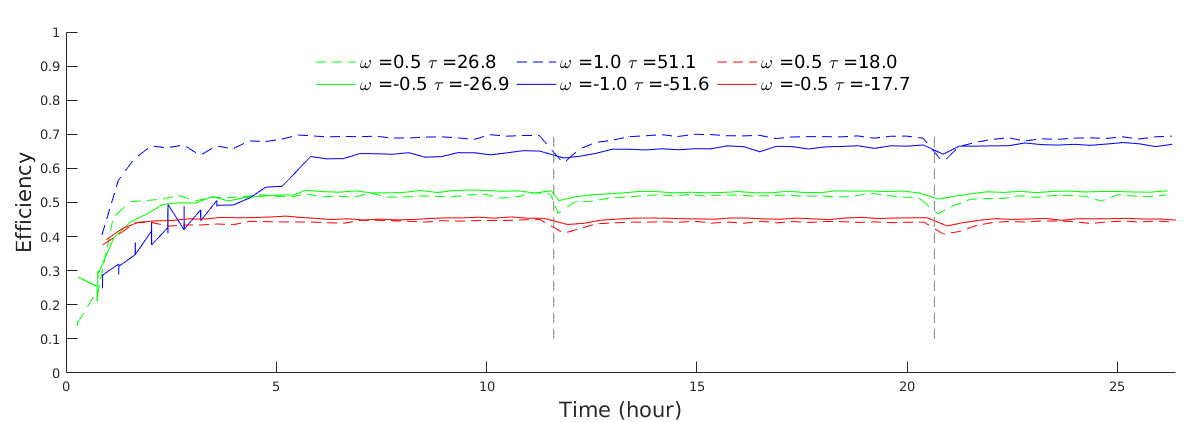
\includegraphics[width=\linewidth]{fig/burn_in}
   \caption{The first three days of testing show a substantial wear-in period for high torque periods.}
   \label{fig:break_in}
\end{figure}
\todo[inline]{fix legend size}

There was a substantial break-in time for the actuator before steady state results were achieved highlighted in Fig \ref{fig:break_in}).
In the high torque case, specifically in the reverse direction, there was an approximately linear increase in efficiency over the course of the first seven hours of duty cycle testing.
This testing began after a minimum of five hours of run time spread out through many short sessions while getting the test system running.
The large increase in efficiency can be noted in the other lower torque profiles as well, starting well below their final steady state values.
The authors theorize that this is due to break-in of the manufactured parts required because of machining inaccuracies.
Due to the complex interaction required of the trochoidal motion profile, slight manufacturing deficiencies could cause build-ups of stress and loss in particular points on the drive.
It would make sense that these could manifest in one direction and not the other if a lobe was misshapen on the trailing edge in one direction, it would be the lead in the other, causing the additional loss.
Through the first hours of testing, these materials likely wore in to each other until the contact was smooth, resulting in the more readily achieved steady state efficiencies in subsequent hours of testing.

Additionally, there is a marked improvement over the first 30 minutes of runtime in the efficiency of the system.
This is likely due to the grease and heat in the system.
The gearbox is greased with Lucas Oil Red'N'Tacky which has a viscosity index of 86 min.
This was chosen because it is designed for high loads for extended periods of time in gear and sliding surface applications, as well as ease of use for Earth testing and verification.
Therefore, during the warm-up period as the actuator temperature increases, the viscosity decrease is likely enough to cause a notable increase in efficiency of the system.
The authors leave the study of a lower viscosity grease's effect on performance, as well as grease suitable for vacuum, for future work.

Finally, through the efficiency comparison after 100 hours of testing (Fig. \ref{fig:eff_results}) and 300 hours of testing (Fig. \ref{fig:eff_results_final}) there was no appreciable loss in efficiency of the system. The actuator maintained a high level of efficiency, 81\% peak, throughout the testing. This result, coupled with the qualitative analysis of the parts after disassembly suggests that the lifetime of this actuator can greatly exceed the current testing of 129k revolutions, which suggests this is a viable actuator for robotic systems where backlash is acceptable and a high reduction and high torque actuator is necessary. 


